\chapter{$^{154}$Gd Results and Discussion}

\section{Ground State Band Confirmation}
\label{sec:154GS_Confirm}

The first lines looked at in the data are the ground state band of $^{154}$Gd. These lines are all pure E2 transitions, making them an excellent diagnostic to compare with theoretical conversion coefficients. The transitions up to the $10^+$ are summarized and compared with theory in Table \ref{tab:154Gd_Single_ICC_GS}.

For the $6^+\rightarrow 4^+$ and $8^+\rightarrow 6^+$ transitions, electron contributions from smaller gamma lines of similar energy had to be subtracted. This was determined by looking at the conversion coefficients of these transitions in gated spectra, as discussed in the next section. In the gated spectra, the internal conversion coefficients were in agreement with theory, meaning the transitions did not have contaminants. To do so, the gamma-ray had been seen and identified with known multipolarity. The conversion coefficient was then assumed from theory, and the contribution to the area was calculated to be

\begin{equation}
    \label{eq:ICC_Subtract}
    A_{e} = \alpha \epsilon_{e} \frac{A_{\gamma}}{\epsilon_{\gamma}} C_{\angle}
\end{equation}

where $\epsilon_{i}$ are the efficiencies of the electrons and gammas. $C_{\angle}$ is the angular correction for this particular transition. Here, it is multiplied, and not divided, so it can be subtracted from the uncorrected area.

The calculated contributions were subtracted off the fitted area of the electron peak, before the conversion coefficient was calculated. This made the error also include contributions from the errors of these gamma peaks and the errors on the theoretical $\alpha$ values. 

There were two types of transitions that acted as contaminants: those of similar energy, and higher energies whose K-electron energies were similar to the L and M peaks of the lines of interest. The peaks are summarized in Table \ref{tab:154Gd_Contaminants}.

\afterpage{\clearpage\begin{landscape}
    \begin{longtable}{c|c|c|c|c|c|c|c|c|c|c}
        \caption{$^{154}$Gd Ground State Band Internal Conversion Coefficients from Singles}
        \label{tab:154Gd_Single_ICC_GS}\\
        \toprule
        $E$ (keV)	&	$J^{\pi}	\rightarrow	J^{\pi}$	&	$E_i$ (keV)	&	$E_f$ (keV)	&	$T_{1/2}$ (fs)	&	Multipolarity & Shell &	$\alpha$ (This Work)				&	$\alpha$  (Th)	&	$\alpha$ (Spits) & $\alpha$ (Gono)		\\
        \hline
        \endfirsthead
        \caption[]{$^{154}$Gd Ground State Band Internal Conversion Coefficients from Singles}\\
        \toprule
        $E$ (keV)	&	$J^{\pi}	\rightarrow	J^{\pi}$	&	$E_i$ (keV)	&	$E_f$ (keV)	&	$T_{1/2}$ (fs)	&	Multipolarity	& Shell &	$\alpha$ (This Work)				&	$\alpha$  (Th)	&	$\alpha$ (Spits) & $\alpha$ (Gono)	\\
        \hline
	    \endhead
	    \hline
        122.23	&	$2^+	\rightarrow	0^+$	&	123.0709	&	0	&	1184000	&	E2	&	K &	0.7759 (34) $^{+148}_{-146}$	&	0.656 (10)	& 0.61 (3) &		\\
    	&				&		&			&		&	& L	&	0.3788 (26) $^{+81}_{-80}$	&	0.411 (6)	&	&	\\
	    &				&		&		&			&	& M	&	0.1323 (3) (29)	&	0.0963 (14)	&	&	\\
	    \hline
        247.85	&	$4^+	\rightarrow	2^+$	&	370.9998	&	123.0709	&	45600	&	E2	&	K &	0.1044	(2) $^{+31}_{-30}$	&	0.1000 (12)	&	0.080 (3)	& 0.0827 (119)\\
	    &				&		&		&		& &	L	&	0.0272	(1) (8)	&	0.0225 (4)	&		\\
	    &				&		&		&		& & M	&	0.0096	(1) (3)	&	0.00513 (8)	&		\\
	    \hline
        346.59$^\dagger$	&	$6^+	\rightarrow	4^+$	&	717.662	&	370.9998	&	8260	&	E2 & K &	0.0335	(1)$^{+11}_{-10}$	&	0.0304 (5)	&	0.029 (1) & 0.0306*	\\
	    &				&		&		&		&	& L	&	0.0087	(1) (3)	&	0.00662 (10)	&		\\
	    &				&		&		&		&	& M	&	0.0027	(1)	(1) &	0.001491 (21)	&		\\
	    \hline
        426.84$^\dagger$	&	$8^+	\rightarrow	6^+$	&	1144.44	&	717.662	&	2570	&	[E2] & K & 0.0180	(2) (5)	&	0.01716 (24)	&	& 0.0170 (22)	\\
    	&				&		&		&		&	& L	&	0.0030	(1) (1)	&	0.00332 (5)	&		\\
	    &				&		&		&		&  	& M	&	0.0008	(1)	(1) &	0.000741 (11)	&		\\
	    \hline
        493.171	&	$10^+	\rightarrow	8^+$	&	1637.05	&	1144.44	&	1110	&	E2	& K	&	0.0124	(4) (4)	&	0.01179 (17)	& &	0.0124 (21)	\\
	    &				&		&		&		&	& L	&	0.0067	(4) (2)	&	0.00213 (3)	&		\\
        \bottomrule
    \end{longtable}
    \item{A list of ground state band conversion coefficients from $^{154}$Gd. Multipolarities and mixing ratios were taken from NNDC. Unless otherwise stated, the $\alpha$ values are $\alpha_K$. An angular distribution correction has been applied based on multipolarities for pure transitions, and those with known mixing ratios. The first error is statistical, the second is systematic. Numbers are compared with Spits et al.\citep{spits96:_154gd} and Gono et al.\citep{gono74:_154gd_e0} The starred value was used as an absolute calibration of the conversion electron detector in the Gono work. The dagger lines had contaminant lines subtracted from the conversion electrons. See the text for more details.}
\end{landscape}}

\afterpage{\clearpage\begin{table}[!]
    \centering
    \begin{longtable}{>{\small}c|>{\small}c|>{\small}c|>{\small}c|>{\small}c|>{\small}c|>{\small}c|>{\small}c}
        \caption{$^{154}$Gd Ground State Band $6^+\rightarrow 4^+$ and $8^+\rightarrow 6^+$ Extra Electron Peak Contributions in Singles}
        \label{tab:154Gd_Contaminants} \\
        \toprule
         $E$ & $E_i$ & $E_f$ & $J_i\rightarrow J_f$ & Multipolarity & $\delta$ & Shell & $\alpha$  \\ \hline
         \endhead
         \endfoot
         \endlastfoot
         \multicolumn{8}{l}{346.59 keV, $6^+\rightarrow 4^+$} \\ \hline
         338.28 & 1770 & 1432 & $5^+_{4^+}\rightarrow 5^+_{\gamma}$ & E0,E2,M1 & -0.004 & K & 0.10 (1) \\ 
         & & & & & $\frac{K(E0)}{K(E2)}\approx 1.0$ & L & 0.01210 (12) \\ 
         & & & & & & M & 0.00180 (3) \\ \hline
         342.18 & 2254 & 1911 & $8^+_{4^+}\rightarrow 6^+_{4^+}$ & E2 & & K & 0.0315 (5) \\ 
         & & & & & & L & 0.0069 (1) \\\
         & & & & & & M & 0.001554 (22) \\ \hline
         390.73 & 1756 & 1366 & $8^+_{0^+_2}\rightarrow 6^+_{0^+_2}$ & E2 & & K & 0.0218 (3) \\ \hline
         \multicolumn{8}{l}{426.84 keV, $8^+\rightarrow 6^+$} \\ \hline
         422.12 & 1418 & 996 & $2^+_{0^+_3}\rightarrow 2^+_{\gamma}$ & E0,E2,M1 & Assumed $\approx 1$ & K & 0.114 (16) \\ 
         & & & & & & L & 0.0161 (23) \\ 
         & & & & & & M & 0.0049 (12) \\ \hline
         466.99 & 1719 & 1251 & $2^-_{2^-}\rightarrow 3^-_{0^-}$ & M1,E2 & Assumed $\approx 1$ & K & 0.019 (6) \\ \hline
         478.27 & 1719 & 1241 & $2^-_{2^-}\rightarrow 1^-_{0^-}$ & E2 & & K & 0.01272 (18) \\
         \bottomrule
         \multicolumn{8}{p{\textwidth}}{Table \ref{tab:154Gd_Contaminants}: A list of the transitions in the $^{154}$Gd Singles data that were contributing to the electron peaks corresponding to the ground state band lines. Conversion coefficients were assumed using BrICC\citep{kibedi08:_BRICC}. The bands for each level are listed as subscripts.}
    \end{longtable}
\end{table}}


\section{Gates on the Ground State Band}
\label{sec:154GS_Gates}

The transitions of the ground state band were the most prominent seen in the gamma-ray and conversion electron spectra. To build a level scheme based on known levels and transitions, these transitions were gated on. Figures \ref{fig:154_2to0}, \ref{fig:154_4to2}, \ref{fig:154_6to4}, and \ref{fig:154_8to6} are the result of these gates. In the cases of cascades, secondary gates were done to confirm assignments.

Determining which transitions went uniquely into a given level was done by comparing the outgoing ground state transition for that level with the incoming transition (i.e. for the $2^+$ level, the 123 keV gate was compared directly with the 247 keV gate). Lines in the gamma spectrum that were present only in the outgoing spectrum, but not the incoming, were assumed to be populating that level.

There were nine bands seen in the gating outside of the ground state band, 4 of which are bands with excited $0^+$ band heads. These are seen in both the $2^+\rightarrow0^+$ gate (Figure \ref{fig:154_2to0}. Three of these bands are seen in the $4^+\rightarrow2^+$ gate (Figure \ref{fig:154_4to2}, and two are seen in the $6^+\rightarrow4^+$ gate (Figure \ref{fig:154_6to4}. Only one is seen in the $8^+\rightarrow6^+$ gate (Figure \ref{fig:154_8to6}. This drop off is not surprising for several reasons, including the lack of known higher spin states in the higher energy $0^+$ bands. The other large reason is the drop off in populating higher energy states in the nucleus.

\begin{figure}[!]
    \centering
    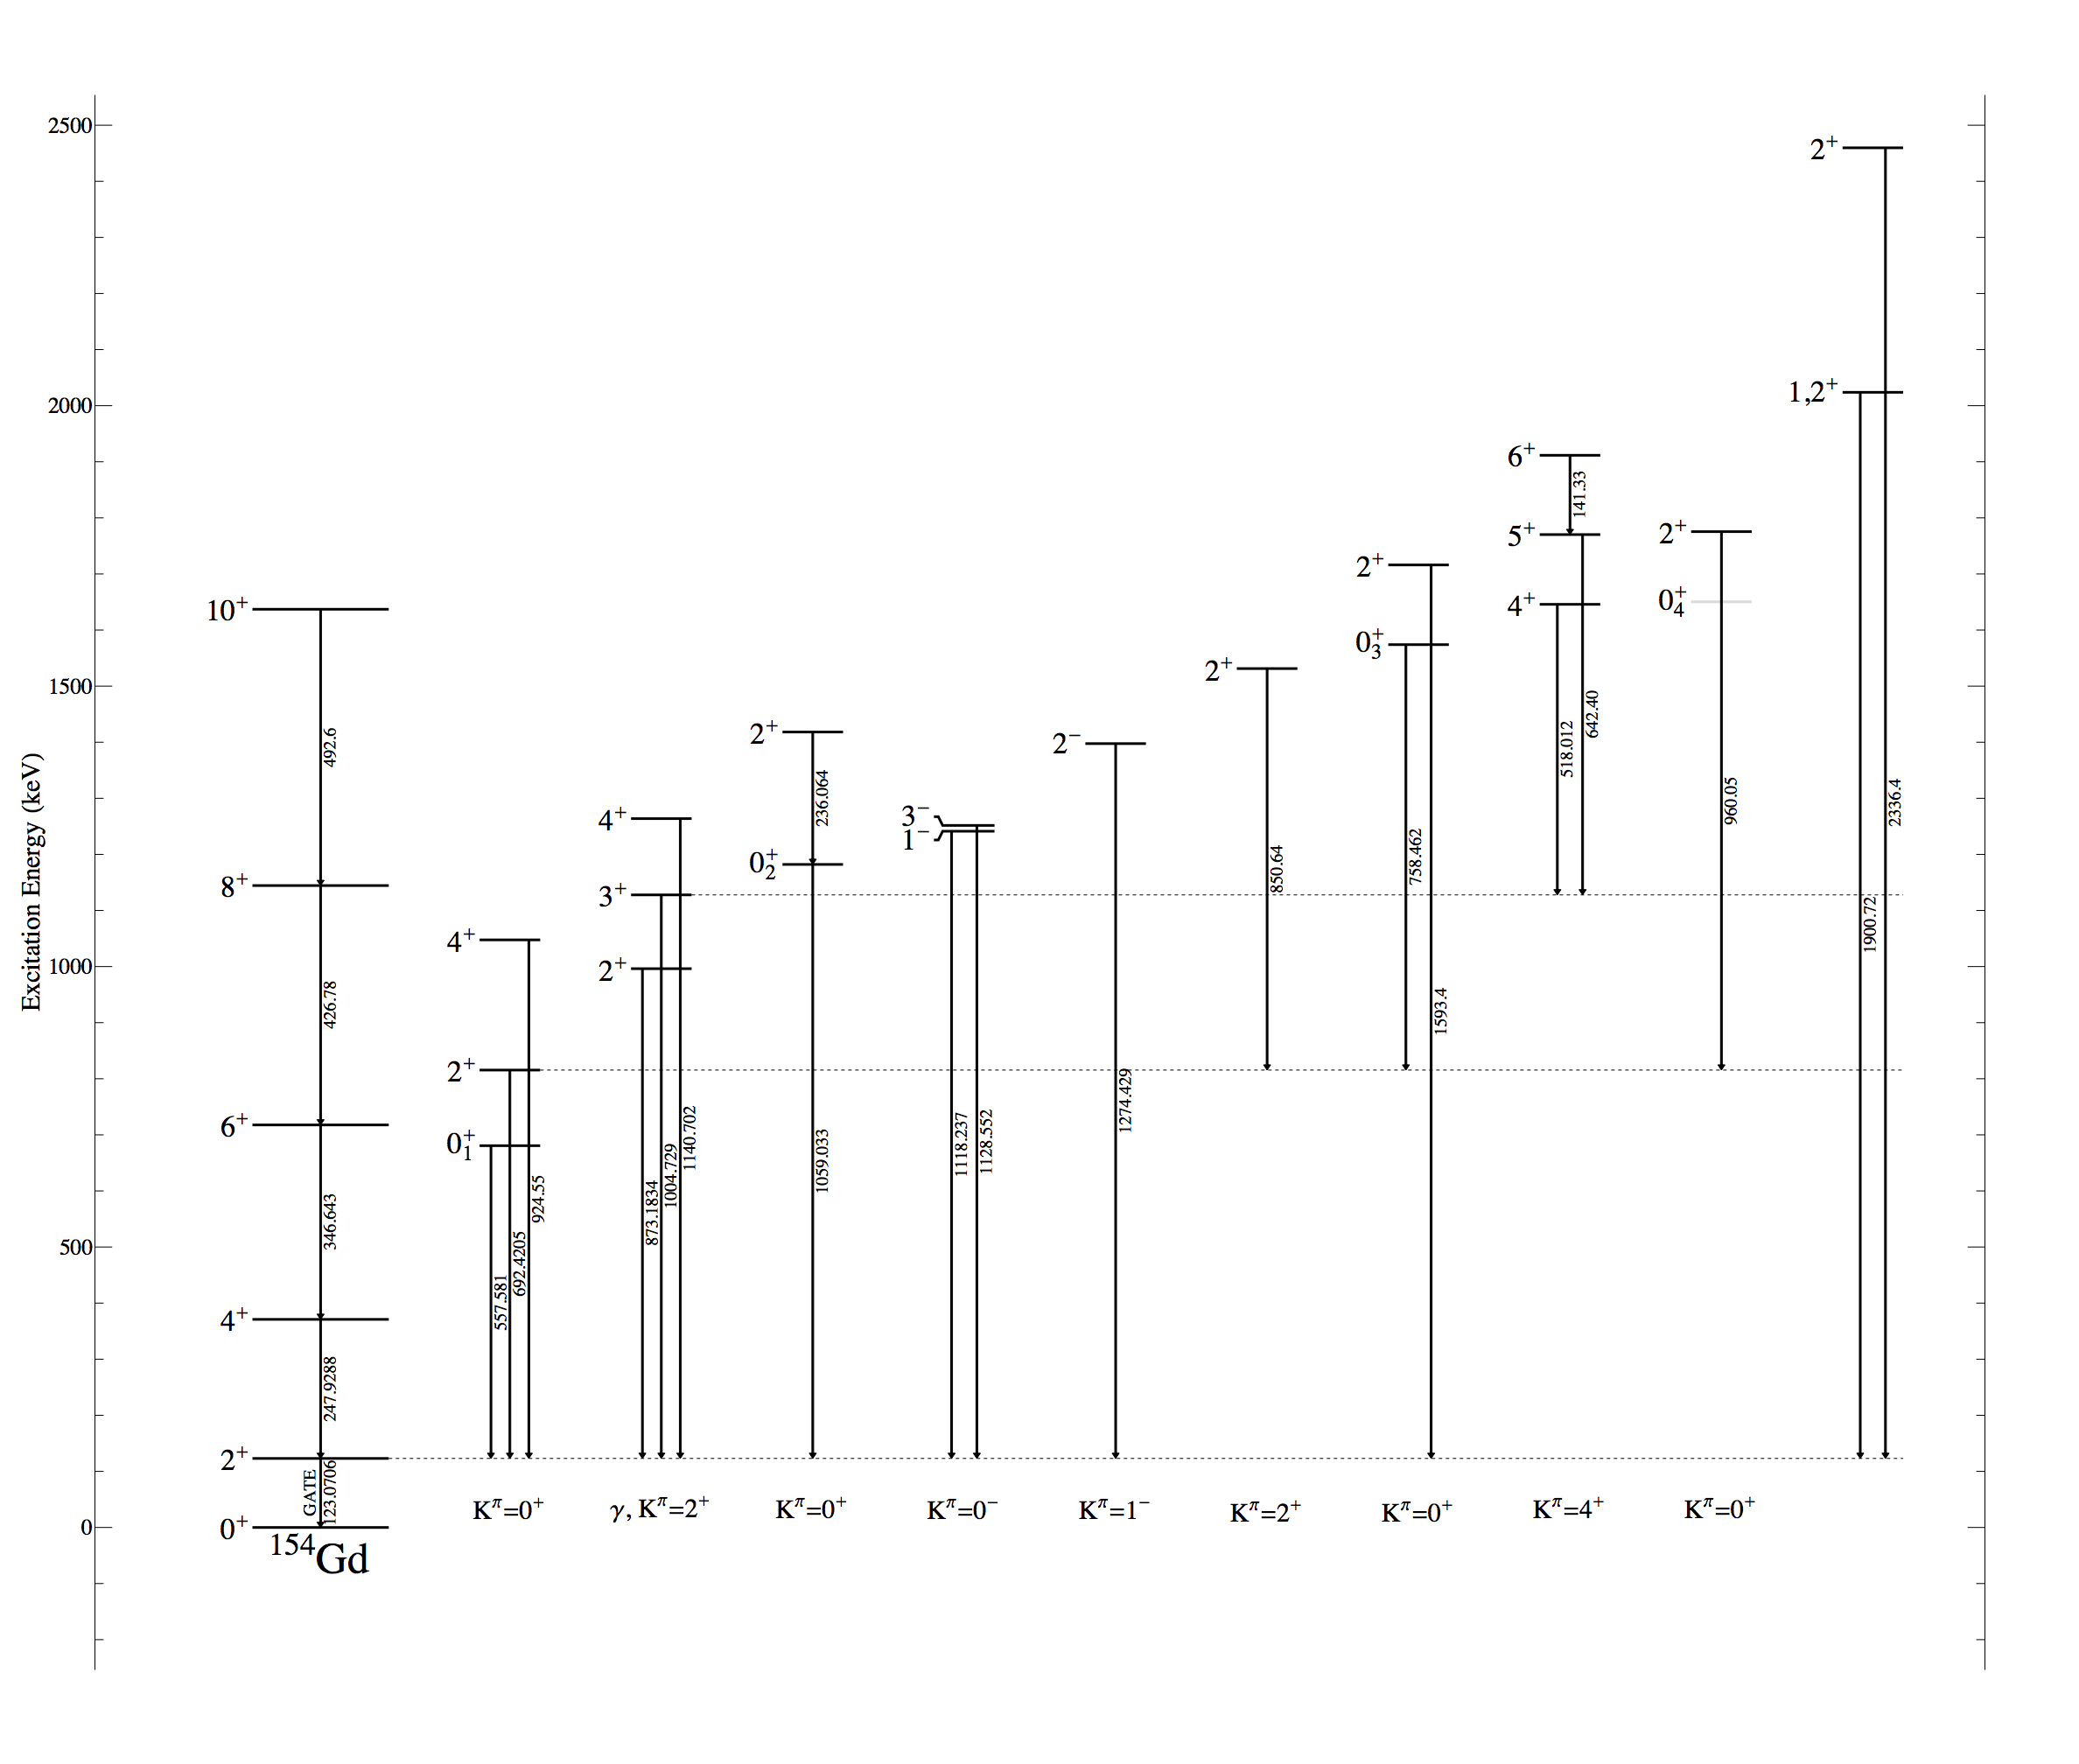
\includegraphics[scale=0.18]{154GdTablesAndFigs/154Gd_2to0.png}
    \caption{Level Scheme of $^{154}$Gd. The gamma ray of the $2^+$\rightarrow$0^+$ transition in the ground state was gated on. It was then compared with the gated spectrum from the gamma ray of the $4^+$\rightarrow$2^+$ transition in the ground state. Peaks only appearing in the first gate were assumed to go into the $2^+$ state, and assignments were made. Due to the low energy of the $2^+$\rightarrow$0^+$ transition, the efficiency was lower, and it is likely that transitions into the $2^+$ state were missed. The levels are organized by band. The lower levels of the band, unseen by gamma rays in this gate, are in gray.}
    \label{fig:154_2to0}
\end{figure}

\begin{figure}[!]
    \centering
    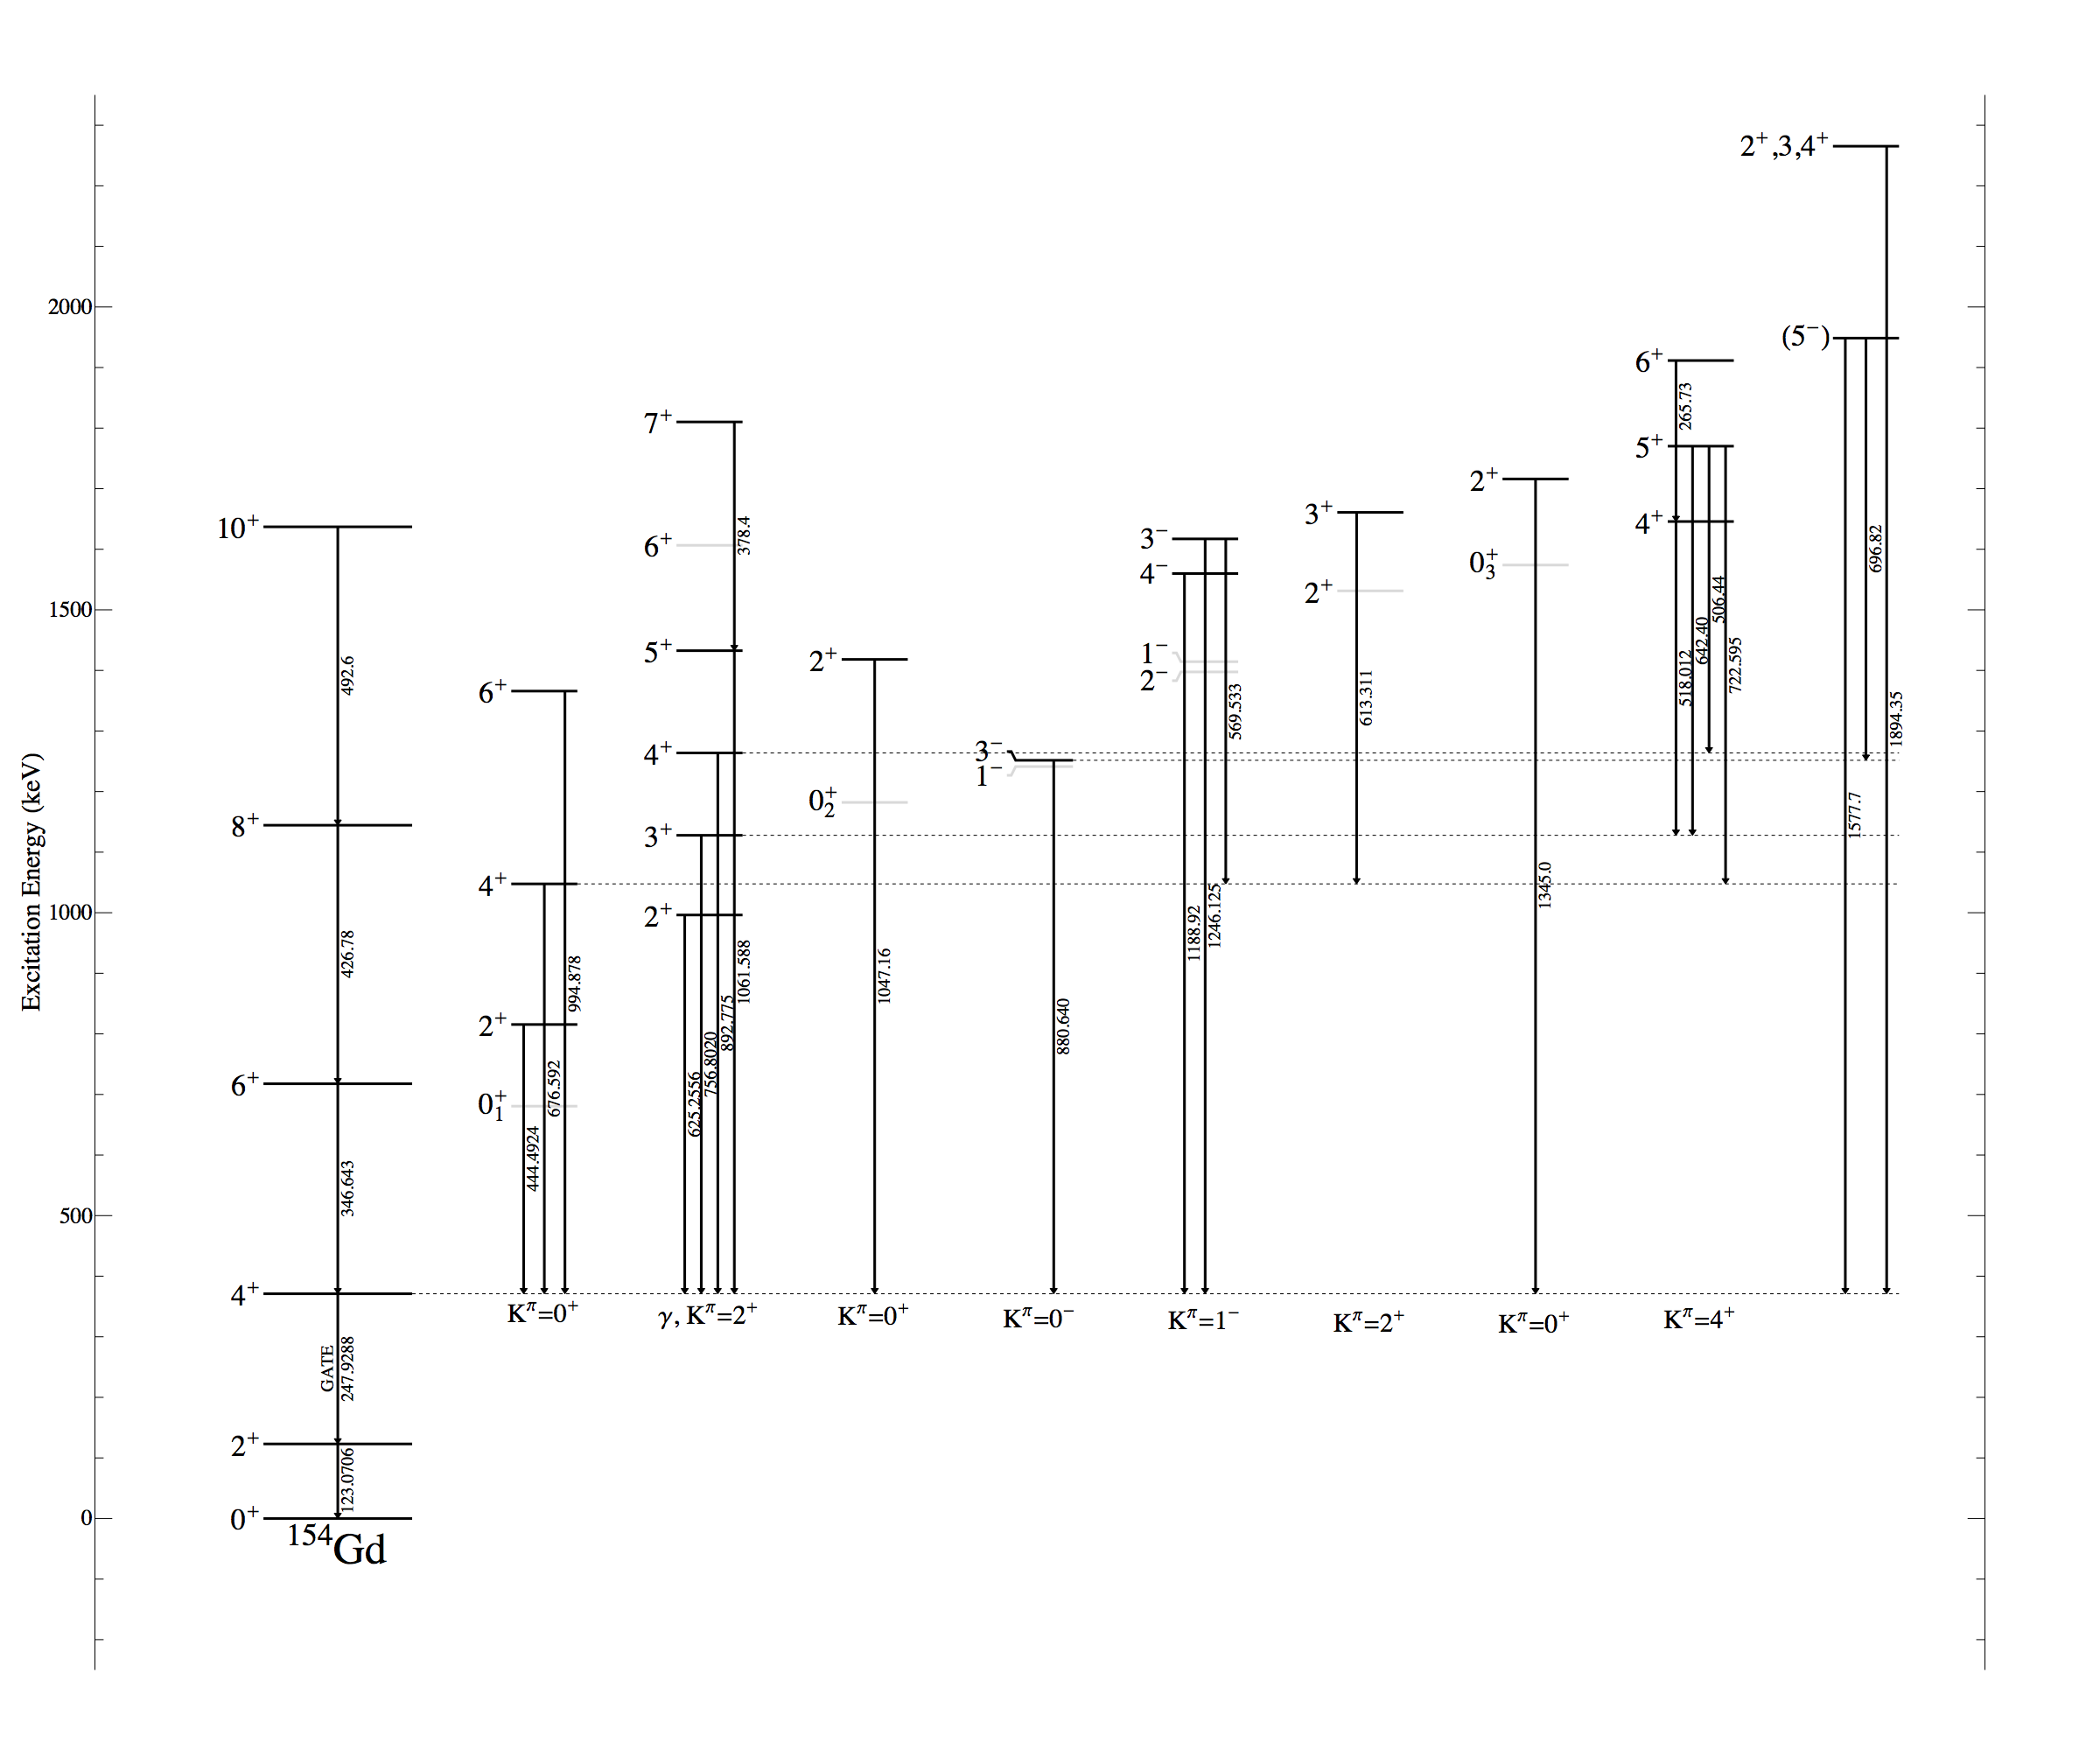
\includegraphics[scale=0.18]{154GdTablesAndFigs/154Gd_4to2.png}
    \caption{Level Scheme of $^{154}$Gd. The gamma ray of the $4^+$\rightarrow$2^+$ transition in the ground state was gated on. It was then compared with the gated spectrum from the gamma ray of the $6^+$\rightarrow$4^+$ transition in the ground state. Peaks only appearing in the first gate were assumed to go into the $4^+$ state, and assignments were made. Additionally, these peaks were also gated on, to look for cascades leading into the $4^+$ state, which were found in several cases. The levels are organized by band. The lower levels of the band, unseen by gamma rays in this gate, are in gray.}
    \label{fig:154_4to2}
\end{figure}

\begin{figure}
    \centering
    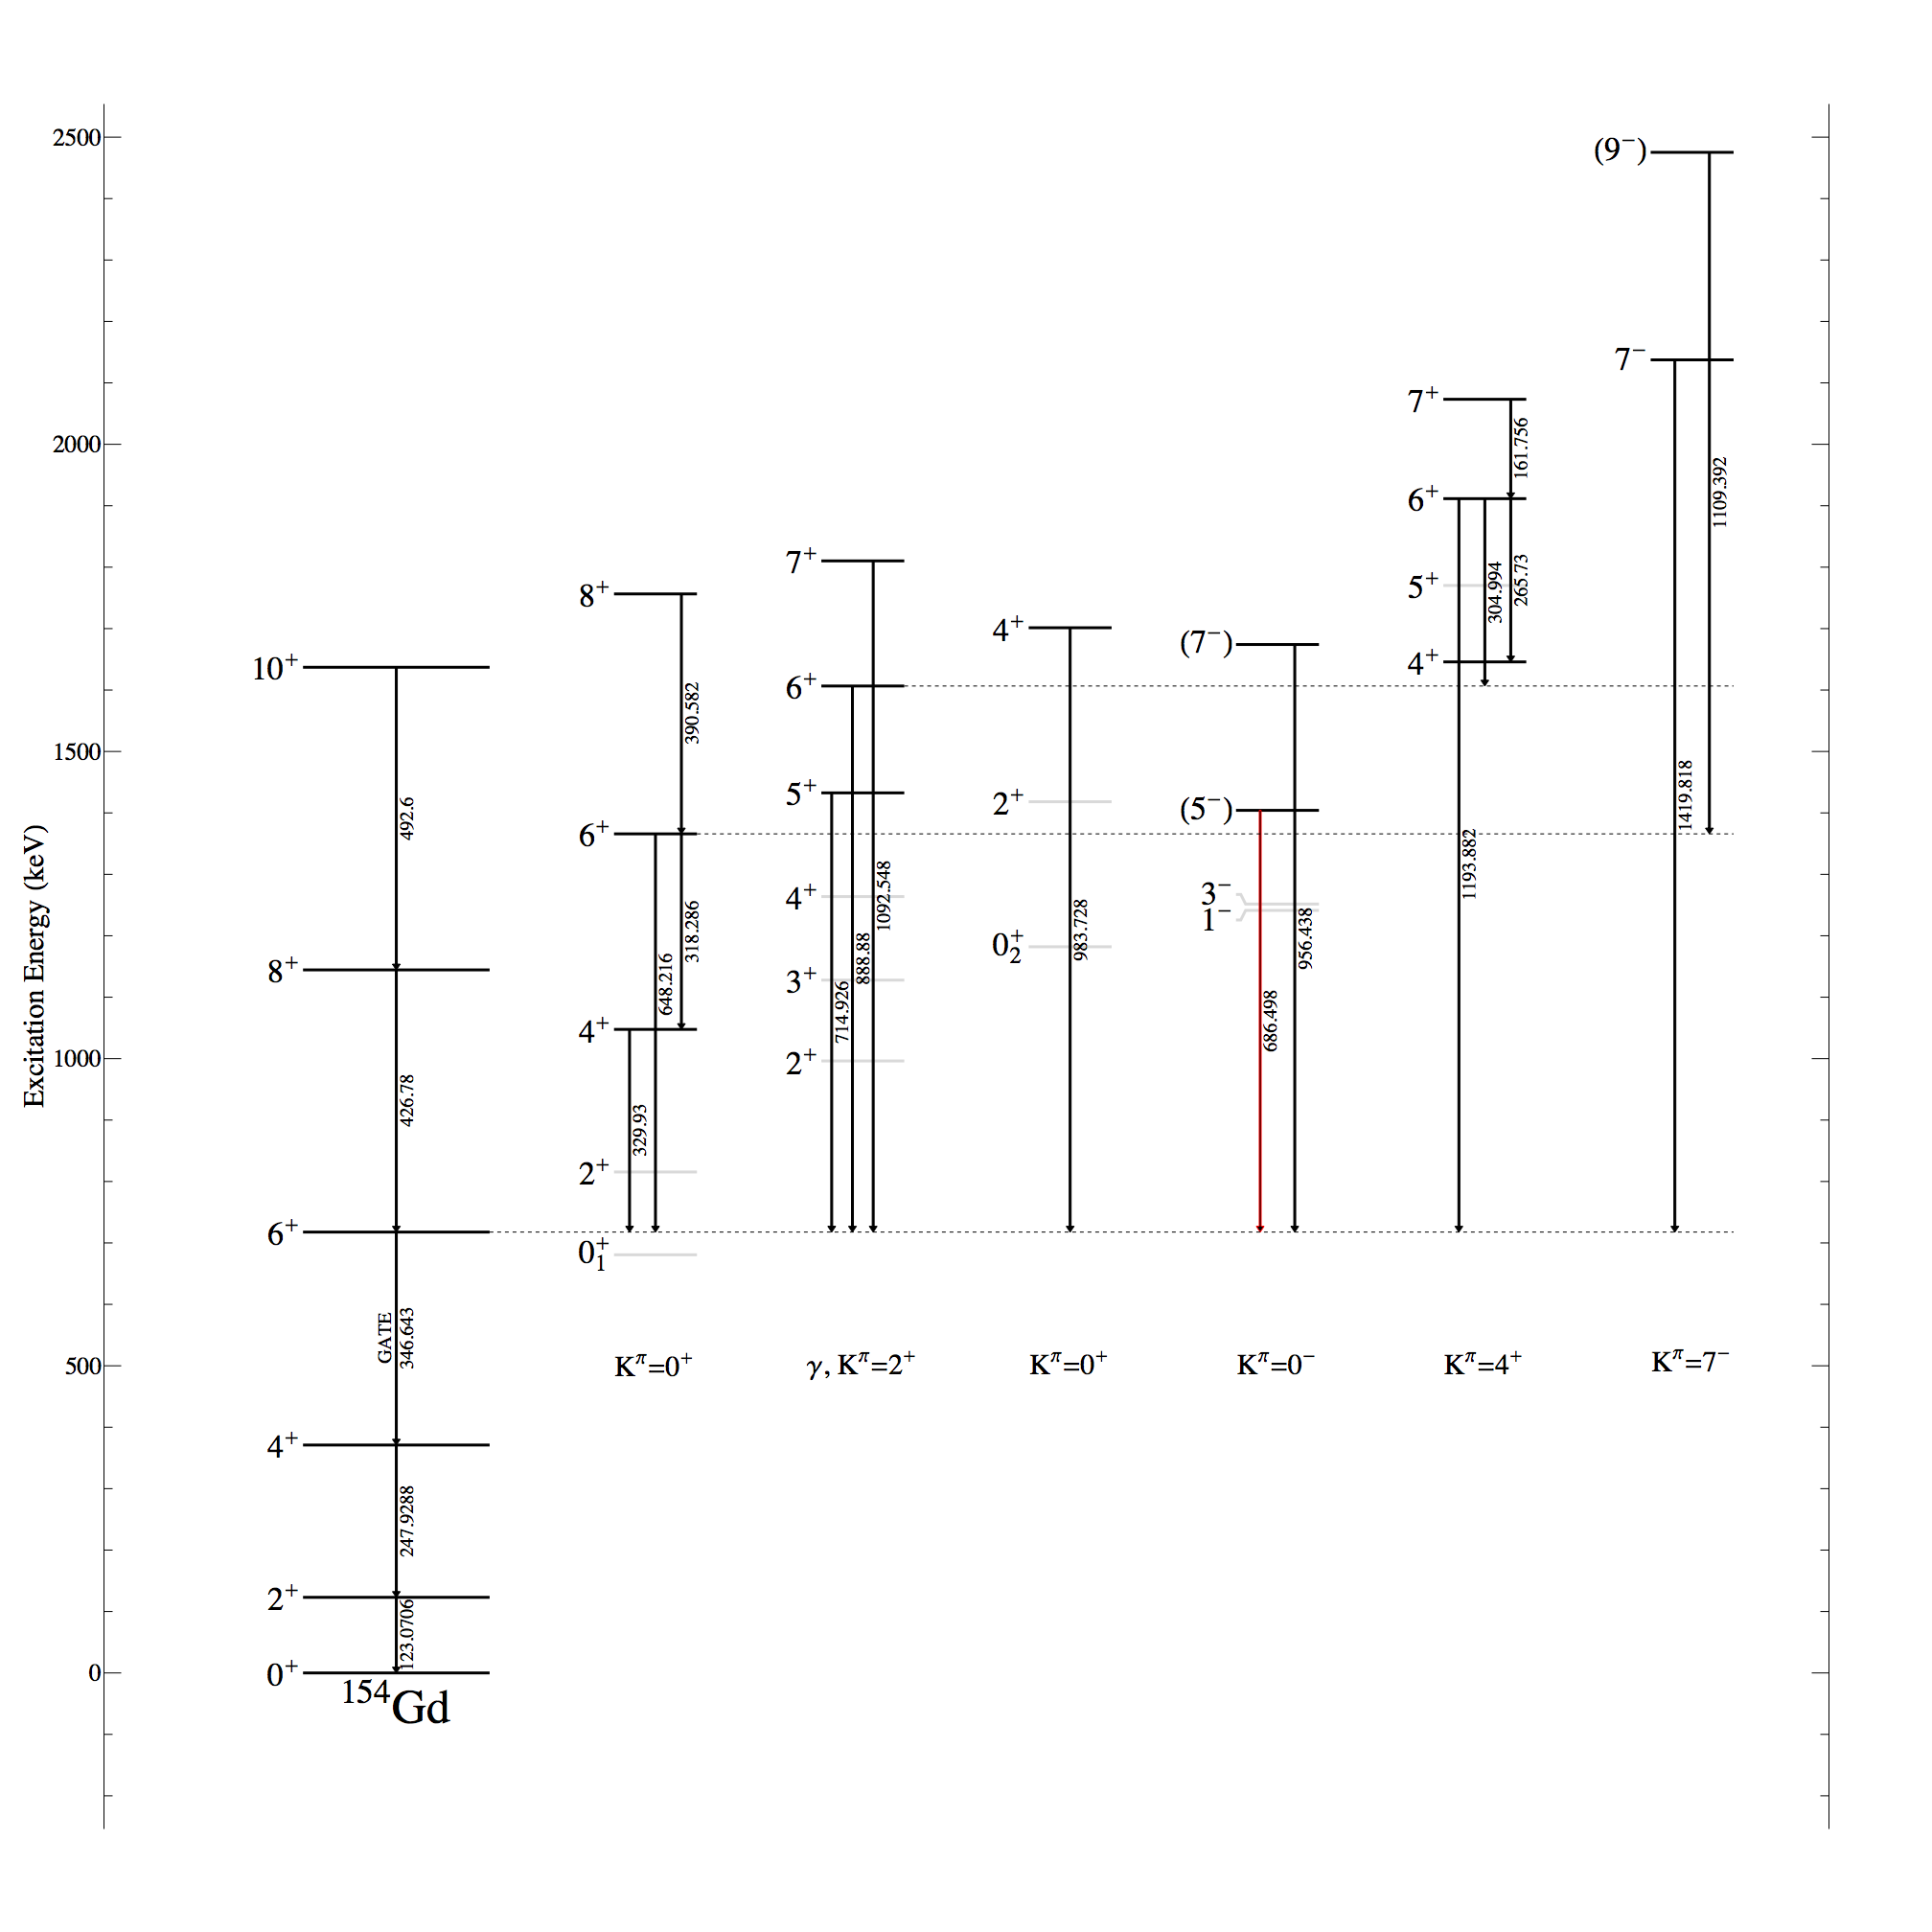
\includegraphics[scale=0.2]{154GdTablesAndFigs/154Gd_6to4.png}
    \caption{Level Scheme of $^{154}$Gd. The gamma ray of the $6^+$\rightarrow$4^+$ transition in the ground state was gated on. It was then compared with the gated spectrum from the gamma ray of the $8^+$\rightarrow$6^+$ transition in the ground state. Peaks only appearing in the first gate were assumed to go into the $6^+$ state, and assignments were made. Additionally, these peaks were also gated on, to look for cascades leading into the $6^+$ state, which were found in several cases. The levels are organized by band. The lower levels of the band, unseen by gamma rays in this gate, are in gray.}
    \label{fig:154_6to4}
\end{figure}

\begin{figure}[!]
    \centering
    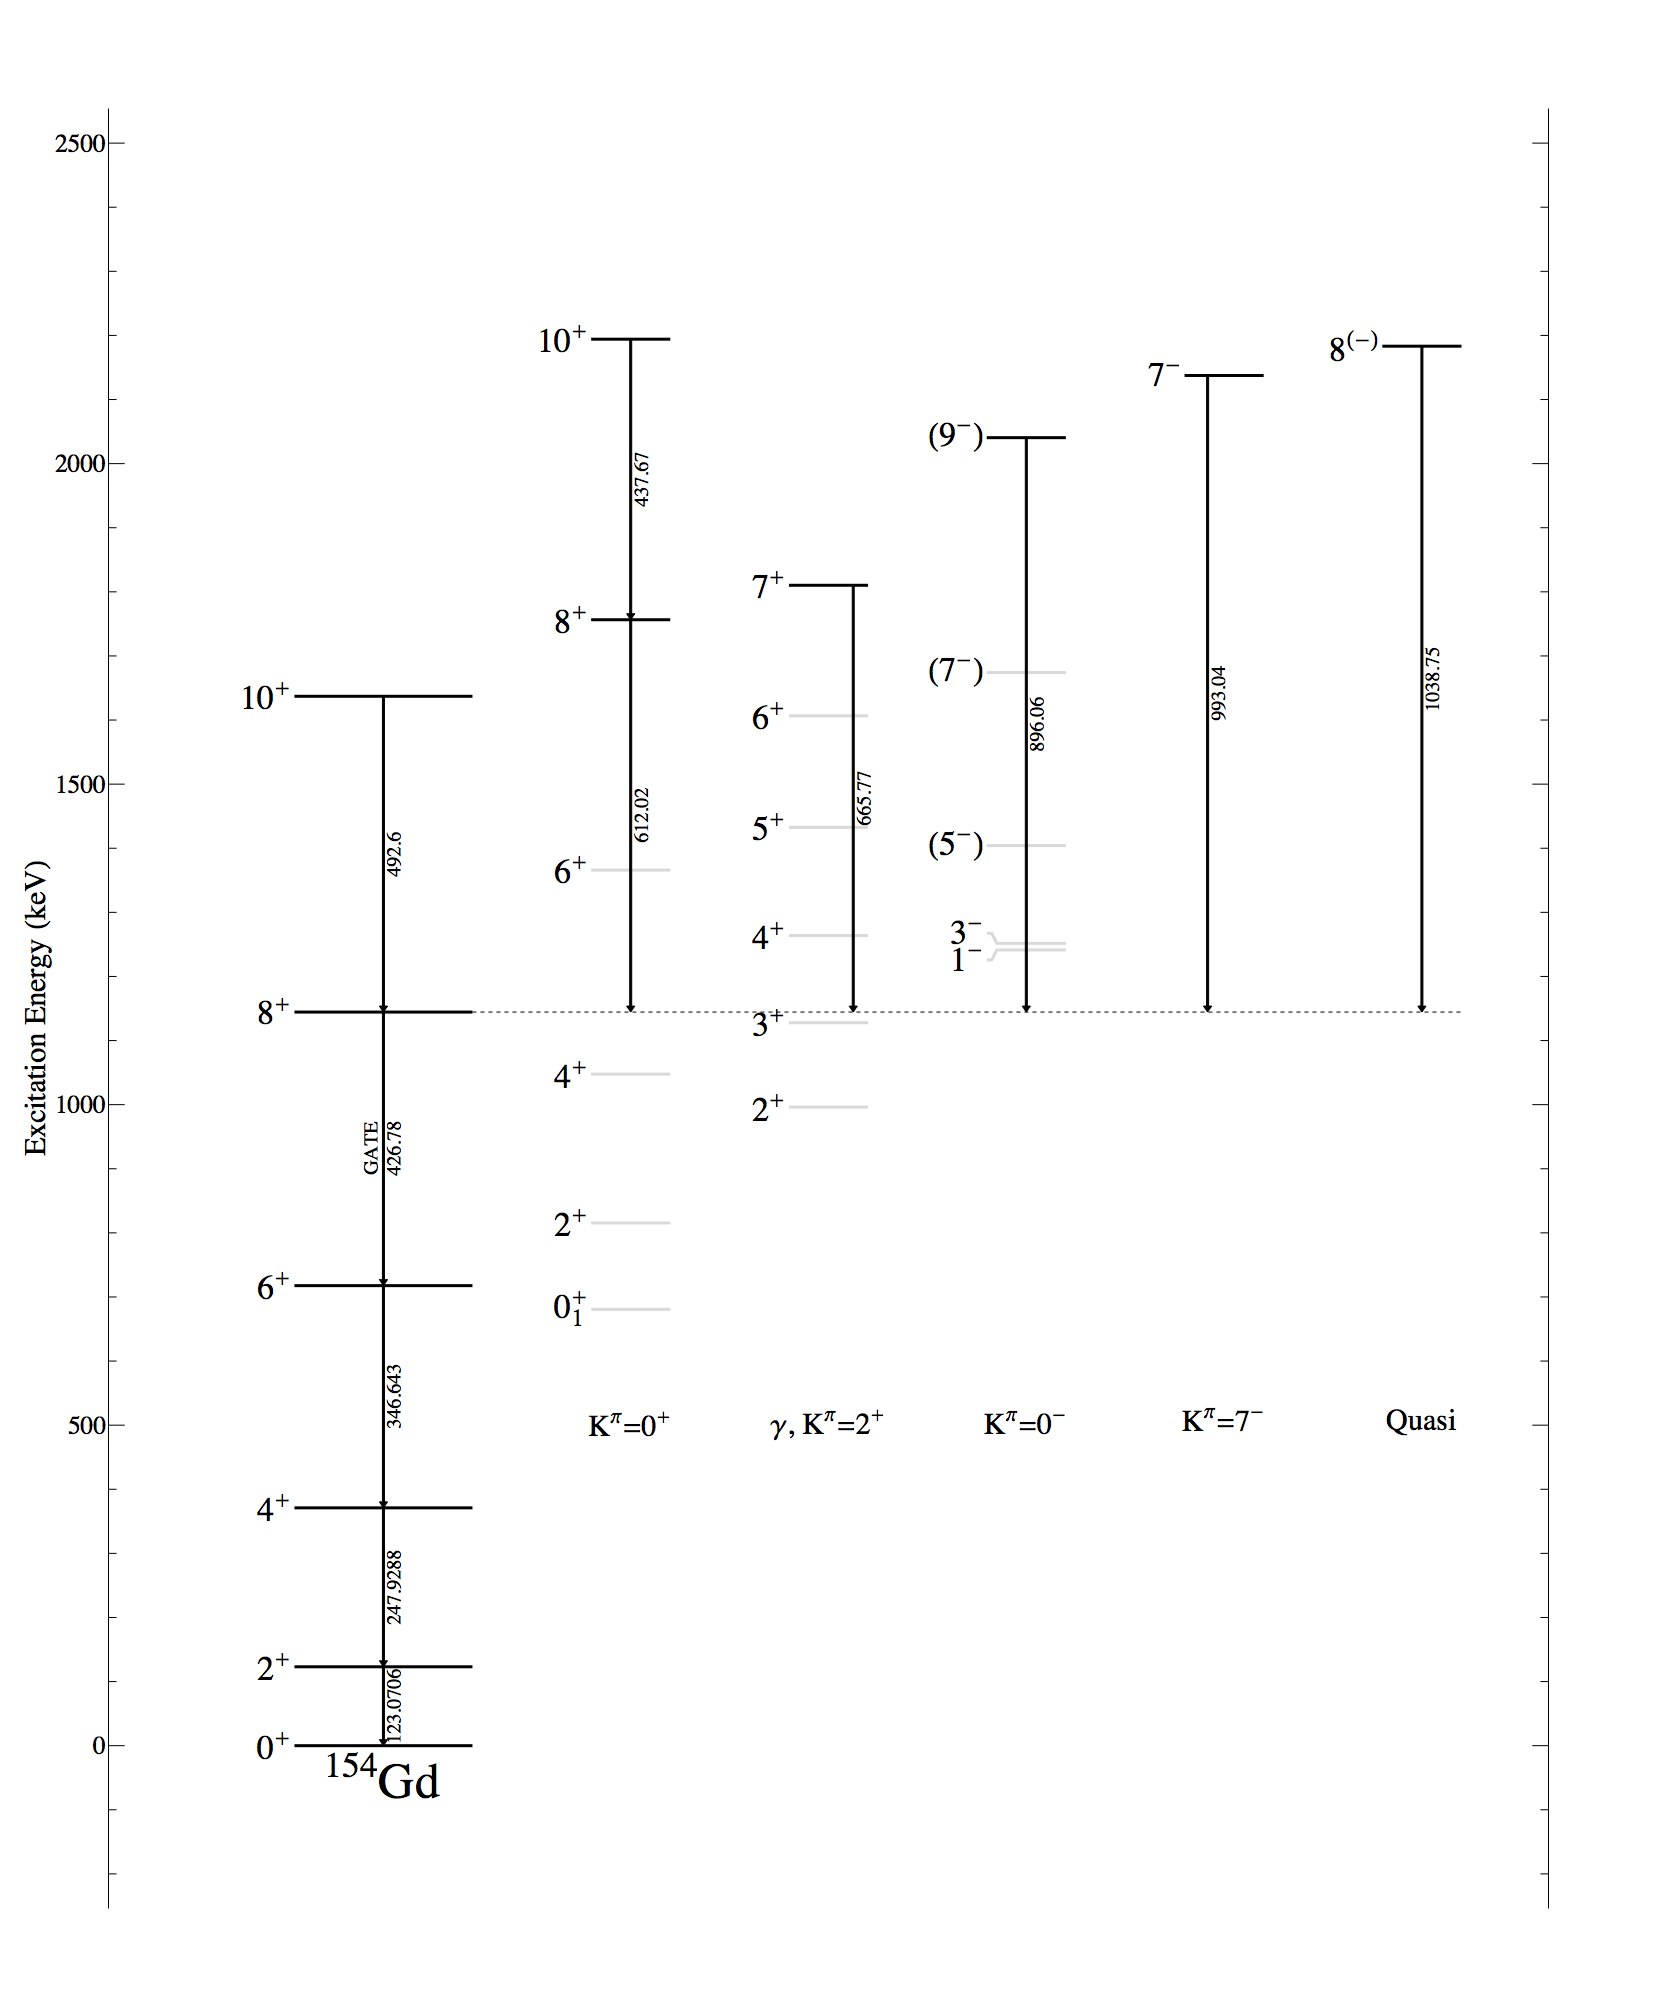
\includegraphics[scale=0.25]{154GdTablesAndFigs/154Gd_8to6.png}
    \caption{Level Scheme of $^{154}$Gd. The gamma ray of the $8^+$\rightarrow$6^+$ transition in the ground state was gated on. It was then compared with the gated spectrum from the gamma ray of the $10^+$\rightarrow$8^+$ transition in the ground state. Peaks only appearing in the first gate were assumed to go into the $8^+$ state, and assignments were made. Additionally, these peaks were also gated on, to look for cascades leading into the $8^+$ state, which were found in several cases. The levels are organized by band. The lower levels of the band, unseen by gamma rays in this gate, are in gray.}
    \label{fig:154_8to6}
\end{figure}

\section{Conversion Coefficients from Singles}
\label{sec:154_Conv_Singles}

\afterpage{\clearpage\begin{table}
    \centering
    \caption{$^{154}$Gd Internal Conversion Coefficients from Singles}
    \label{tab:154Gd_Single_ICC}
\begin{ThreePartTable}
    \begin{tabular}{c|c|c|c|c|c|c}
        \multicolumn{7}{>{\fontsize{12}{15}}c}{(a)}\\
        \toprule
        $E$ (keV)	&	$J^{\pi}	\rightarrow	J^{\pi}$	&	$E_i$ (keV)	&	$E_f$ (keV)	&	$T_{1/2}$ (fs)	&	Multipolarity	&	$\delta$\\
        \hline
        232.44	&	$4^+_{0^+_2}	\rightarrow	2^+_{0^+_2}$	&	1047.592	&	815.4917	&	7600	&	E2	&	\\
	    &				&		&		&		&		& \\
	    \hline
        329.49	&	$4^+_{0^+_2}	\rightarrow	6^+_{gs}$	&	1047.592	&	717.662	&	7600	&	E2	&	\\
        \hline
        349.89	&	$2^+_{2^+_2}	\rightarrow	0^+_{gs}$	&	1531.305	&	1182.091	&		&	[E2]	&	 \\
        \hline
        416.79	&	$4^+_{0^+_6}	\rightarrow	3^+_{2^+_2}$	&	2080.23	&	1660.903	&		&	(M1)	&	\\
        \hline
        444.19	&	$2^+_{0^+_2}	\rightarrow	4^+_{\gamma}$	&	815.4917	&	370.9998	&	6400	&	E2	&		\\
        \hline
        506.41	&	$5^+_{4^+_1}	\rightarrow	4^+_{\gamma}$	&	1770.187	&	1263.778	&		&	E2	&		\\
        \hline
        515.92	&	$4^+_{4^+_1}	\rightarrow	3^+_{\gamma}$	&	1645.814	&	1127.802	&		&	E2+M1	&	-7 (3)	\\
        \hline
        557.58	&	$0^+_{0^+_2}	\rightarrow	2^+_{gs}$	&	680.6673	&	123.0709	&	4560	&	E2	&		\\
        \hline
        610.71	&	$8^+_{0^+_2}	\rightarrow	8^+_{gs}$	&	1756.49	&	1144.44	&		&	E0+M1+E2	&	-0.69 (14)	\\
	    &				&		&		&		&		&	\\
	    \hline
        676.70	&	$4^+_{0^+_2}	\rightarrow	4^+_{gs}$	&	1047.592	&	370.9998	&	7600	&	E0+M1+E2	&	+2.9 (4)	\\
        \hline
        693.47	&	$2^+_{0^+_2}	\rightarrow	2^+_{gs}$	&	815.4917	&	123.0709	&	6400	&	E2+M1+E0	&	7.5 (4)	\\
        \hline
        873.54	&	$2^+_{\gamma}	\rightarrow	2^+_{gs}$	&	996.2568	&	123.0709	&	950	&	E2+M1+E0	&	-9.4 (4)	\\
        \hline
        889.61	&	$6^+_{\gamma}	\rightarrow	6^+_{gs}$	&	1606.55	&	717.662	&		&	E2+M1	&	$>1.8$	\\
        \hline
        894.40	&	$4^+_{\gamma}	\rightarrow	4^+_{gs}$	&	1263.778	&	370.9998	&		&	E0+M1+E2	&	-3.8 (3)	\\
        \hline
        924.85	&	$4^+_{0^+_2}	\rightarrow	2^+_{gs}$	&	1047.592	&	123.0709	&	7600	&	E2	&	\\
        \hline
        996.33	&	$2^+_{\gamma}	\rightarrow	0^+_{gs}$	&	996.2568	&	0	&	950	&	E2	&	\\
        \hline
        1005.12	&	$3^+_{\gamma}	\rightarrow	2^+_{gs}$	&	1127.8018	&	123.0709	&		&	E2+M1	&	-7.4 (4) \\
        \bottomrule
    \end{tabular}
    \end{ThreePartTable}
\end{table}
\begin{table}
    \begin{ThreePartTable}
        \begin{tabular}{c|c|c|c|c|c}
            \multicolumn{6}{>{\fontsize{12}{15}}c}{TABLE 4.3 (CONTINUED)}\\
            \multicolumn{6}{>{\fontsize{12}{15}}c}{(b)}\\
            \toprule
            $E$ (keV) & Shell &	$\alpha$ (This Work)	&	$\alpha$  (Theory)\citep{kibedi08:_BRICC}	&	$\alpha$ (Spits)\citep{spits96:_154gd} & $\alpha$ (Gono)\citep{gono74:_154gd_e0}		\\
            \hline
            232.44	& K &	0.287	(103) $^{+83}_{-82}$	&	0.0982 (14)	&	0.100 (8)	\\
            &	LM &		0.0450	(46) (13)	&	0.0288 (4)	&		\\
            \hline
            329.49	 & K &	0.1573	(89) (17)	&	0.0352 (5)	&	0.034 (3)	\\
            \hline
            349.89	& K &	0.0298 (8) $^{+8}_{-7}$	&	0.0296 (5)	& $<0.097$ &		\\
            \hline
            416.79	 & K &	0.0334	(47) (6)	&	0.03442 (5)	&	\\
            \hline
            444.19	& K &	0.0525	(32) (6)	&	0.01543 (22)	&	0.014 (1)	\\
            \hline
            506.41	& K &	0.0071	(4) (1)	&	0.01098 (16)	&	0.0100 (11)	\\
            \hline
            515.92	& K & 	0.0069	(5) (1)	&	0.0107 (4)	&	0.0113 (9)	\\
            \hline
            557.58	& K &	0.0486	(42) (6)	&	0.00864 (12)	&	0.009 (1) & 0.0091 (16)	\\
            \hline
            610.71	& K &	0.0258	(10) (7)	&	0.0110 (6)	& &	0.053 (7)	\\
            		& L &	0.0167	(9) (4)	&	0.00158 (7)	&		\\
            \hline
            676.70	& K &	0.0283	(4) (10)	&	0.00593 (17)	&	0.0460 (46) & 0.040 (7)	\\
            \hline
            693.47	& K &	0.0017	(2) (1)	&	0.00522 (8)	&	0.0421 (4)	\\
            \hline
            873.54	& K &	0.0021	(3)	(1) &	0.00311 (5)	&	0.0035 (1)	\\
            \hline
            889.61	& K &	0.0043	(6) (2)	&	0.00349 (5)	&	0.0033 (2)	\\
            \hline
            894.40	& K &	0.0019	(2) (1)	&	0.00307 (5)	&	0.0039 (3)	\\
            \hline
            924.85	& K &	0.0033	(9) (1)	&	0.00273 (4)	&	0.0031 (1)	\\
            \hline
            996.33	& K &	0.0021	(4) (1)	&	0.00234 (4)	&	0.0025 (1)	\\
            \hline
            1005.12	& K &	0.0019	(1) (1)	&	0.00233 (4)	&	0.0024 (1)	\\
            \bottomrule
        \end{tabular}
        \begin{tablenotes}[para]
            Table \ref{tab:154Gd_Single_ICC}: A list of conversion coefficients from $^{154}$Gd. Table (a) lists transition information. Multipolarities and mixing ratios were taken from the nuclear data sheets\citep{reich09:_nds_154}. Table (b) lists the conversion coefficients. Unless otherwise stated, the $\alpha$ values are $\alpha_K$. An angular distribution correction has been applied based on multipolarities for pure transitions, and those with known mixing ratios. The first error is statistical, the second is systematic. Numbers are compared with Spits et al.\citep{spits96:_154gd} and Gono et al.\citep{gono74:_154gd_e0} The starred value was used as an absolute calibration of the conversion electron detector in the Gono work. The bands for each level are listed as subscripts.
        \end{tablenotes}
\end{ThreePartTable}
\end{table}
}

\afterpage{\clearpage\begin{sidewaystable}
\footnotesize
    \begin{longtable}{c|c|c|c|c|c|c|c|c|c|c}
        \caption{Uncorrected $^{154}$Gd Internal Conversion Coefficients from Singles}
        \label{tab:154Gd_Single_ICC_Uncorr}\\
        \toprule
        $E$ (keV)	&	$J^{\pi}	\rightarrow	J^{\pi}$	&	$E_i$ (keV)	&	$E_f$ (keV)	&	Multipolarity	&	$\delta$ & Shell	&	$\alpha$ (This Work)				&	$\alpha$  (Th)	&	$\alpha$ (Spits) & $\alpha$ (Gono)		\\
        \hline
        \endfirsthead
        \caption[]{Uncorrected $^{154}$Gd Internal Conversion Coefficients from Singles}\\
        \toprule
        $E$ (keV)	&	$J^{\pi}	\rightarrow	J^{\pi}$	&	$E_i$ (keV)	&	$E_f$ (keV)	&	Multipolarity	&	$\delta$ & Shell	&	$\alpha$ (This Work) 			&	$\alpha$  (Th)	&	$\alpha$ (Spits) & $\alpha$ (Gono)	\\
        \hline
	    \endhead
	    \hline
        198.311	&	$3^-	\rightarrow	2^+$	&	1617.123	&	1418.16		&	[E1]	&		& K &	0.0842	(26) (19)	&	0.0393 (6)	&		\\
	    &	$(9)^+	\rightarrow	(8)^+$	&	2453.29	&	2254.12		&		&		&					&		&	&	\\
	    \hline
        313.21	&	$3^+	\rightarrow	2^+$	&	1127.802	&	815.492		&	[M1,E2]	&	 & K	&	0.0805	(47) (20)	&		&		\\
        \hline
        641.92	&	$5^+	\rightarrow	3^+$	&	1770.187	&	1127.8018		&	M1,E2	&		& K &	0.0303 (7) (8)	&		&	0.0086 (8)	\\
        648.951	&	$6^+	\rightarrow	6^+$	&	1365.87	&	717.662		&	E0+M1+E2	&	+1.30 (20)	&		&	0.0079 (5)	&	& 0.039 (7)	\\
        \hline
        715.198	&	$2^+	\rightarrow	2^+$	&	1531.305	&	815.492		&	E0+M1+E2	&		& K &	0.0199	(5) (5)	&		&	0.0070 (5)	\\
	    &				&		&			&		&		& L &	0.0041	(4) (1)	&		&		\\
	    \hline
        1061.59	&	$0^+	\rightarrow	2^+$	&	1182.091	&	123.0709		&	E2	&		& K &	0.0022	(3) (1)	&	0.0021 (1)	&		\\
	    &	$5^+	\rightarrow	4^+$	&	1432.588	&	370.9998		&	E2+M1	&	$-4.3^{+12}_{-26}$	&			&	0.0021 (1)	&	0.0019 (4) & &	\\
        \bottomrule
    \end{longtable}
    \item{Table \ref{tab:154Gd_Single_ICC_Uncorr}: A list of conversion coefficients from $^{154}$Gd. Multipolarities and mixing ratios were taken from NNDC. Unless otherwise stated, the $\alpha$ values are $\alpha_K$. No angular distribution correction has been applied, either due to unknown mixing ratios, or multiple assignments of the gamma-ray. None of the above transitions have known half-lives. The first error is statistical, the second is systematic. Numbers are compared with Spits et al.\citep{spits96:_154gd} and Gono et al.\citep{gono74:_154gd_e0}}
\end{sidewaystable}}

\afterpage{\clearpage\begin{landscape}
\begin{table}
    \centering
    \caption{$^{154}$Gd Internal Conversion Electrons without Assigned Multipolarities}
    \label{tab:154Gd_No_Mult_ICC}
\begin{ThreePartTable}
        \centering
    \begin{tabular}{>{\footnotesize}c|>{\footnotesize}c|>{\footnotesize}c|>{\footnotesize}c}
        \multicolumn{4}{>{\fontsize{12}{15}}c}{(a)}\\
        \toprule
        $E$ (keV) & $J_i\rightarrow J_f$	& $E_i$ (keV) 	& $E_f$ (keV) \\
	    \hline
	    266.37	&	$6^+_{4^+_1}	\rightarrow	4^+_{4^+_1}$	&	1911.544	&	1645.814 \\ \hline
	    303.89	&	$(7^+)_{4^+_1}	\rightarrow	5^+_{4^+_1}$	&	2073.30	&	1770.187 \\ \hline
	    318.382	&	$6^+_{0^+_2}	\rightarrow	4^+_{0^+_2}$	&	1365.87	&	1047.592	\\
	    &		&		&		\\  \hline
	    379.55	&	$7^+_{\gamma}	\rightarrow	5^+_{\gamma}$	&	1810.21	&	1432.588 \\ \hline
        433.12	&	$4^+_{0^+_6}	\rightarrow	4^+_{4^+_1}$	&	2080.23	&	1645.814	\\ 
        	&	&	&	\\ \hline
        687.05	&	$(5^-)_{0^-} \rightarrow 6^+_{gs}$		&	1404.16	&	717.662 \\ \hline
        722.64	&	$5^+_{4^+_1}	\rightarrow	4^+_{0^+_2}$	&	1770.187	&	1047.592 \\
        &	&	&	\\ \hline
        1033.91	&	$3^-	\rightarrow	4^+_{0^+_2}$	&	2080.791	&	1047.592 \\
        \bottomrule
    \end{tabular}
\end{ThreePartTable}
\end{table}

\begin{table}
    \centering
\begin{ThreePartTable}
    \centering
    \begin{tabular}{>{\footnotesize}c|>{\footnotesize}c|>{\footnotesize}c|>{\footnotesize}c|>{\footnotesize}c|>{\footnotesize}c|>{\footnotesize}c|>{\footnotesize}c}
        \multicolumn{7}{>{\fontsize{12}{15}}c}{TABLE 4.5 (CONTINUED)}\\
        \multicolumn{7}{>{\fontsize{12}{15}}c}{(b)}\\
        \toprule
        &	& \multicolumn{2}{>{\footnotesize}c|}{$\alpha$ (This Work) } & \multicolumn{3}{>{\footnotesize}c|}{Theory\citep{kibedi08:_BRICC}}	& 	\\ 
        $E$ (keV)	& Shell & 	Uncorrected & Corrected 	& $\alpha$(M1) & $\alpha$(E2) & $\alpha$(E1) &	$\alpha$ (Spits)\citep{spits96:_154gd}	\\
	    \hline
	    266.37	& K &	0.2074	(74) (50) & 0.1684 (60) (41) &  & 0.0654 (10) & & \\ \hline
	    303.89	& K &	0.1183	(40) $^{+30}_{-29}$  & 0.0954 (32) $^{+24}_{-23}$ & & 0.0444 (7) & & \\ \hline
	    318.382	& K &	0.0736	(18) (18)  & 0.0600 (15) (15) & & 0.0388 (6) & &\\
	    		& L & 	0.0371	(12) (9) & 0.0301 (10) (7)	& & 0.00892 (13) & &	\\  \hline
	    379.55	& K & 	0.1120	(60) (31) & 0.0903 (48) (25)&  & 0.0236 (4) & & \\ \hline
        433.12	& K &	0.0571	(42) (15) & [M1] 0.0777 (57) (20) & 0.0310 (5) & 0.01650 (24) &	& 0.0220 (45)\\ 
        	&	& & [E2] 0.0351 (26) (9) & & &	& \\ \hline
        687.05	& K & 0.3538 (116) (90) & 0.6435 (211) (163)	& & & 0.00203 (3) &\\ \hline
        722.64	& K		&	0.0166	(12) (42) & [M1] 0.0107 (8) (27)	& 0.00856 (12) & 0.00468 (7) & &		\\
        &	& &  [E2] 0.0185 (13) (47) & & &	& \\ \hline
        1033.91	& K	&	0.0015	(4) (1) & 0.0028 (7) (2)	& & & 0.000916 (13) &	\\
        \bottomrule
    \end{tabular}
\begin{tablenotes}[para]
    Table \ref{tab:154Gd_No_Mult_ICC}: A list of conversion coefficients from $^{154}$Gd without known multipolarities. Table (a) lists transition information. Table (b) lists the conversion coefficients and theoretical values. As a result, an angular distribution correction term cannot be applied to compare with theory, except in the case of pure multipoles. None of the above transitions have known half-lives. The first error is statistical, the second is systematic. Numbers are compared with theoretical coefficients for allowed and reasonable polarities, as well as results from Spits et al. \cite{spits96:_154gd} The bands for each level are listed as subscripts. The $3^-$ for $E=1033.91$ keV has no band placement.
    \end{tablenotes}
\end{ThreePartTable}
\end{table}
\end{landscape}}   

\afterpage{\clearpage\begin{sidewaystable}
    \begin{longtable}{c|c|c|c|c|c|c|c}
        \caption{$0^+\rightarrow 0^+$ Transitions in $^{154}$Gd}
        \label{tab:154Gd_0_to_0}\\
        \toprule
        &	& 	&  &	& \multicolumn{2}{c|}{Theory}	& 	\\ 
        $E_i$ (keV)	&	$E_f$ (keV)	& $E$ (keV)	&	Gate &		$\alpha$ (This Work)	& $\alpha$(M1) & $\alpha$(E2) &	$\alpha$ (Spits)	\\
        \hline
        \endfirsthead
        \toprule
        \caption[]{$0^+\rightarrow 0^+$ Transitions in $^{154}$Gd}\\
        &	& 	&  &	& \multicolumn{2}{c|}{Theory}	& 	\\ 
        $E_i$ (keV)	&	$E_f$ (keV)	& $E$ (keV)	&	Gate &		$\alpha$ (This Work)	& $\alpha$(M1) & $\alpha$(E2) &	$\alpha$ (Spits)	\\
        \hline
	    \endhead
	    1182.091 & 680.6673 &  501.427 & 557.581 & $>0.0283$ & 0.0213 (3) & 0.01126 (16) & $>0.2$ \\\hline
        1573.9 & 680.6673 &  893.9 & 557.581 & $>0.0183$ & 0.00510 (8) & 0.00294 (5) & \\\hline
        1573.9 & 1182.091 &  391.9 &  1059.033 & $>0.0529$ & 0.0402 (6) & 0.0216 (3) & $>0.1$ \\\hline
        1650.3 & 1182.091 &  468.3 &  1059.033 & $>0.0922$ & 0.0254 (4) & 0.01343 (19) & \\\hline
        1650.3 & 680.6673 &  970.3 & 557.581 & $>0.0209$ & 0.00419 (6) & 0.00247 (4) & $>0.027$ \\
        \bottomrule
	\end{longtable}
    \item{A list of conversion coefficients from $^{154}$Gd for $0^+\rightarrow 0^+$ transitions seen in the gated data. All are lower limits. Numbers are compared with Spits et al.\citep{spits96:_154gd} and theoretical coefficients for M1 and E2 transitions. All coefficients are K-electrons.}
\end{sidewaystable}}

\afterpage{\clearpage\begin{landscape}
    \small
    \begin{longtable}{c|c|c|c|c|c|c|c}
        \caption{$2^+\rightarrow 2^+$ Transitions in $^{154}$Gd}
        \label{tab:154Gd_2_to_2}\\
        \toprule
        &	& 	&  &	& \multicolumn{2}{c|}{Theory}	&	\\ 
        $E_i$ (keV)	&	$E_f$ (keV)	& $E$ (keV)	&	Gate &		$\alpha$ (This Work)	& $\alpha$(M1) & $\alpha$(E2) &	$\alpha$ (Spits)	\\
        \hline
        \endfirsthead
        \caption[]{$2^+\rightarrow 2^+$ Transitions in $^{154}$Gd}\\
        \toprule
        &	& 	&  &	& \multicolumn{2}{c|}{Theory}	&	\\ 
        $E_i$ (keV)	&	$E_f$ (keV)	& $E$ (keV)	&	Gate &		$\alpha$ (This Work)	& $\alpha$(M1) & $\alpha$(E2) &	$\alpha$ (Spits)	\\
        \hline
	    \endhead
	    \endfoot
	    \multicolumn{8}{p{1.2\textwidth}}{Table \ref{tab:154Gd_2_to_2}: A list of conversion coefficients from $^{154}$Gd for $2^+\rightarrow 2^+$ transitions seen in the gated data. The first error is statistical, the second is systematic. Numbers are compared with theoretical K-shell conversion coefficients for M1 and E2 transitions, as well as results from Spits et al.\citep{spits96:_154gd} All coefficients are K-electrons.}
	    \endlastfoot
        815.4917 & 123.0709 &  692.4205 & 123.0706 &  0.0430 (3) (9) & 0.00952 (14) & 0.00516 (8) &  0.0421 (4)\\ \hline
        996.264 & 815.4917 & 180.72 &  692.4205 & $>1.0570$ & 0.320 (5) & 0.210 (3) &  \\
        &  &  & 444.4924 & $>0.9718$ & & &  \\ \hline
        1418.16 & 815.4917 & 602.688 &  692.4205 & $>0.0125$ & 0.01343 (19) & 0.00715 (10) & 0.025 (3)  \\
        &  &  & 444.4924 & $>0.0093$ &  & &\\ \hline
        1418.16 & 996.2568 & 421.893 & 873.1834 & $>0.0367$ & 0.0332 (5) & 0.01170 (25) & 0.114 (16) \\
        &  &  & 625.2556 & $>0.0463$ & & & \\ \hline
        1531.305 & 815.4917 & 715.819 &  692.4205 & 0.0146 (40)$^{+43}_{-33}$ & 0.00877 (13) & 0.00478 (7) & 0.0070 (4)  \\
        &  & & 444.4924 & $0.0234 (80) ^{+68}_{-52}$ & & &\\ \hline
        1531.305 & 996.2568 & 535.050 & 873.1834 & 0.0204 (70)$^{+54}_{-41}$ & 0.0181 (3) & 0.00956 (14) & 0.093 (11)  \\
        & & & 625.2556 & $>0.0183$ & & & \\ \hline
        1716.050 & 815.4917 & 900.5583 &  692.4205 & $<0.0105$ & 0.00501 (7) & 0.00289 (4) &  \\
        & & & 444.4924 & $<0.0531$ & & &  \\ \hline
        1716.050 & 996.2568 & 719.80 & 873.1834 & 0.0113 (46)$^{+33}_{-25}$ & 0.00865 (13) & 0.00472 (7) & \\
        &  &  & 625.2556 & 0.0501 (260)$^{+147}_{-113}$ & & &  \\ \hline
        1775.429 & 815.4917 & 960.05 &  692.4205 & $>0.0221$ & 0.00430 (6) & 0.00253 (4) &  \\
        &  &  & 444.4924 & $>0.0231$ & & &  \\ \hline
        1775.429 & 996.2568 & 779.165 & 873.1834 & 0.0206 (112)$^{+60}_{-46}$ & 0.00712 (10) & 0.00396 (6) & \\
        &  &  & 625.2556 & 0.0745 (521)$^{+217}_{-165}$	& & & \\
        \bottomrule
    \end{longtable}
\end{landscape}}

\afterpage{\clearpage\begin{landscape}
    \small
    \begin{longtable}{c|c|c|c|c|c|c|c|c}
        \caption{$4^+\rightarrow 4^+$ Transitions in $^{154}$Gd}
        \label{tab:154Gd_4_to_4}\\
        \toprule
        &	& 	&  &	& \multicolumn{2}{c|}{Theory}	& & 	\\ 
        $E_i$ (keV)	&	$E_f$ (keV)	& $E$ (keV)	&	Gate &		$\alpha$ (This Work)	& $\alpha$(M1) & $\alpha$(E2) &	$\alpha$ (Spits) & $\alpha$ (Gono)	\\
        \hline
        \endfirsthead
        \caption[]{$4^+\rightarrow 4^+$ Transitions in $^{154}$Gd}\\
        &	& 	&  &	& \multicolumn{2}{c|}{Theory}	& &	\\ 
        $E_i$ (keV)	&	$E_f$ (keV)	& $E$ (keV)	&	Gate &		$\alpha$ (This Work)	& $\alpha$(M1) & $\alpha$(E2) &	$\alpha$ (Spits) & $\alpha$ (Gono)	\\
        \hline
	    \endhead
        1047.592 & 370.9998 &  676.593 & 247.9288 & 0.0550 (2)$^{+12}_{-11}$ & 0.01007 (15) & 0.00544 (8) & 0.0460 (46) & 0.040 (7)\\
        &  &  &  & 0.0131 (1) (3) & 0.001384 (20) & 0.000870 (13) & & \\ \hline
        1263.778 & 1047.592 & 216.186 & 676.593 & $<0.1250$ & 0.196 (3) & 0.1222 (18) &  \\
         &  &  & 924.55 & $<0.1033$ & & &  \\ \hline
        1645.814 & 1047.592 & 598.22 & 676.593 &  $<0.0092$ &  0.01368 (20) & 0.00728 (11) & $<0.067$  \\
         &  &  & 924.55 &  $<0.0142$ & & & \\ \hline
        1645.814 & 1263.778 & 382.025 & 892.775 & $<0.0360$ & 0.0429 (6) & 0.0232 (4) & 0.033 (5) \\
         &  &  & 1140.702 & $<0.0494$ & & & \\ \hline
        1701.39 & 815.4917 & 653.7 & 676.593 & $<0.0093$ & 0.01097 (16) & 0.00590 (9) & 0.0220 (62)  \\
        &  &  & 924.55 & $<0.0301$ & & & \\ \hline
        1701.39 & 1263.778 & 437.612 & 892.775 & $<0.0585$ & 0.0302 (5) & 0.01605 (23) &   \\
        &  &  & 1140.702 & $<0.0511$ & & &   \\ \hline
        1789.17 & 815.4917 & 740.91 & 676.593 & $<0.0124$ & 0.00806 (12) & 0.00443 (7) & \\
        &  &  & 924.55 & $<0.0447$ & & &  \\ \hline
        1789.17 & 1263.778 & 525.392 & 892.775 & $<0.0168$ & 0.0190 (3) & 0.01001 (14) &  \\
        &  &  & 1140.702 & $<0.0161$ & & &  \\
        \bottomrule
    \end{longtable}
    \item{A list of conversion coefficients from $^{154}$Gd for $4^+\rightarrow 4^+$ transitions seen in the gated data. The first error is statistical, the second is systematic. Numbers are compared with theoretical K-shell conversion coefficients for M1 and E2 transitions, as well as results from Spits et al.\citep{spits96:_154gd} and Gono et al.\citep{gono74:_154gd_e0} All coefficients are K-electrons.}
\end{landscape}}

\afterpage{\clearpage\begin{landscape}
    \small
    \begin{longtable}{c|c|c|c|c|c|c|c}
        \caption{$6^+\rightarrow 6^+$ Transitions in $^{154}$Gd}
        \label{tab:154Gd_6_to_6}\\
        \toprule
        &	& 	&  &	& \multicolumn{2}{c|}{Theory}	& 	\\ 
        $E_i$ (keV)	&	$E_f$ (keV)	& $E$ (keV)	&	Gate &		$\alpha$ (This Work)	& $\alpha$(M1) & $\alpha$(E2) &	$\alpha$ (Gono)	\\
        \hline
        \endfirsthead
        \toprule
        \caption[]{$6^+\rightarrow 6^+$ Transitions in $^{154}$Gd}\\
        &	& 	&  &	& \multicolumn{2}{c|}{Theory}	& 	\\ 
        $E_i$ (keV)	&	$E_f$ (keV)	& $E$ (keV)	&	Gate &		$\alpha$ (This Work)	& $\alpha$(M1) & $\alpha$(E2) &	$\alpha$ (Gono)	\\
        \hline
    	\endhead
    	\endfoot
    	\multicolumn{8}{p{1.15\textwidth}}{Table \ref{tab:154Gd_6_to_6}: A list of conversion coefficients from $^{154}$Gd for $6^+\rightarrow 6^+$ transitions seen in the gated data. The first error is statistical, the second is systematic. Numbers are compared with theoretical K-shell conversion coefficients for M1 and E2 transitions, as well as results from Gono et al.\citep{gono74:_154gd_e0} All coefficients are K-electrons.}
    	\endlastfoot
        1365.878 & 717.662 & 648.3 & 346.643 & 0.0778 (4) (16) & 0.01120 (16) & 0.00601 (9) & 0.039 (7)\\ \hline
        1606.55 & 1365.878 & 240.672 & 648.3 & $>0.9065$ & 0.1462 (21) & 0.0885 (13) &  \\
        &  &  & 994.9 & $>1.1070$ & & &  \\ \hline
        1911.544 & 1365.878 & 545.7 & 648.3 &  $<0.0209$ & 0.01723 (25) & 0.00911 (13) &   \\
        &  &  & 994.9 &  $<0.0189$ &  & &  \\ \hline
        1911.544 & 1606.55 & 304.75 & 888.69 & $<0.0794$ & 0.0777 (11) & 0.0440 (7) & 0.042 (6) \\
        \bottomrule
    \end{longtable}
\end{landscape}}
    